% Hlavicka pro protokoly z fyzikalniho praktika.
% Verze pro: LaTeX
% Verze hlavicky: 22. 2. 2007
% Autor: Ustav fyziky kondenzovanych latek
% Ke stazeni: www.physics.muni.cz/ufkl/Vyuka/
% Licence: volne k pouziti, nejlepe k vcasnemu odevzdani protokolu z Vaseho mereni.

\documentclass[a4paper,11pt]{article}

% Kodovani (cestiny) v dokumentu: cp1250
% \usepackage[cp1250]{inputenc}	% Omezena stredoevropska kodova stranka, pouze MSW.
\usepackage[utf8]{inputenc}	% Doporucujeme pouzivat UTF-8 (unicode).
\usepackage{subfig}
\usepackage{float}

\usepackage{xparse}

\NewDocumentCommand{\codeword}{v}{%
\texttt{\textcolor{codepurple}{#1}}%
}

%%% Nemente:
\usepackage[margin=2cm]{geometry}
\newtoks\jmenopraktika \newtoks\jmeno \newtoks\datum
\newtoks\obor \newtoks\skupina \newtoks\rocnik \newtoks\semestr
\newtoks\cisloulohy \newtoks\jmenoulohy
\newtoks\tlak \newtoks\teplota \newtoks\vlhkost
%%% Nemente - konec.


%%%%%%%%%%% Doplnte pozadovane polozky:

\jmenopraktika={Fyzikální praktikum 1}  % nahradte jmenem vaseho predmetu
\jmeno={Milan Suk}            % nahradte jmenem mericiho
\datum={7. května 2018}        % nahradte datem mereni ulohy
\obor={F}                     % nahradte zkratkou vami studovaneho oboru
\skupina={PO 8:00}            % nahradte dobou vyuky vasi seminarni skupiny
\rocnik={I}                  % nahradte rocnikem, ve kterem studujete
\semestr={II}                 % nahradte semestrem, ve kterem studujete

\cisloulohy={4}               % nahradte cislem merene ulohy
\jmenoulohy={Měření gravitační konstanty a tíhového zrychlení} % nahradte jmenem merene ulohy

\tlak={97,9}                   % nahradte tlakem pri mereni (v hPa)
\teplota={21,4}               % nahradte teplotou pri mereni (ve stupnich Celsia)
\vlhkost={40}               % nahradte vlhkosti vzduchu pri mereni (v %)

%%%%%%%%%%% Konec pozadovanych polozek.


%%%%%%%%%%% Uzitecne balicky:
\usepackage[czech]{babel}
\usepackage{graphicx}
\usepackage{amsmath}
\usepackage{xspace}
\usepackage{url}
\usepackage{indentfirst}
\usepackage{listings}
\usepackage{color}


\definecolor{codegreen}{rgb}{0,0.6,0}
\definecolor{codegray}{rgb}{0.5,0.5,0.5}
\definecolor{codepurple}{rgb}{0.58,0,0.82}
\definecolor{backcolour}{rgb}{0.95,0.95,0.92}
 
\lstdefinestyle{mystyle}{
    backgroundcolor=\color{backcolour},   
    commentstyle=\color{codegreen},
    keywordstyle=\color{magenta},
    numberstyle=\tiny\color{codegray},
    stringstyle=\color{codepurple},
    basicstyle=\footnotesize,
    breakatwhitespace=false,         
    breaklines=true,                 
    captionpos=b,                    
    keepspaces=true,                 
    numbers=left,                    
    numbersep=5pt,                  
    showspaces=false,                
    showstringspaces=false,
    showtabs=false,                  
    tabsize=2
}
 
\lstset{style=mystyle}

%%%%%% Zamezeni parchantu:
\widowpenalty 10000 \clubpenalty 10000 \displaywidowpenalty 10000
%%%%%% Parametry pro moznost vsazeni vetsiho poctu obrazku na stranku
\setcounter{topnumber}{3}	  % max. pocet floatu nahore (specifikace t)
\setcounter{bottomnumber}{3}	  % max. pocet floatu dole (specifikace b)
\setcounter{totalnumber}{6}	  % max. pocet floatu na strance celkem
\renewcommand\topfraction{0.9}	  % max podil stranky pro floaty nahore
\renewcommand\bottomfraction{0.9} % max podil stranky pro floaty dole
\renewcommand\textfraction{0.1}	  % min podil stranky, ktery musi obsahovat text
\intextsep=8mm \textfloatsep=8mm  %\intextsep pro ulozeni [h] floatu a \textfloatsep pro [b] or [t]

% Tecky za cisly sekci:
\renewcommand{\thesection}{\arabic{section}.}
\renewcommand{\thesubsection}{\thesection\arabic{subsection}.}
% Jednopismenna mezera mezi cislem a nazvem kapitoly:
\makeatletter \def\@seccntformat#1{\csname the#1\endcsname\hspace{1ex}} \makeatother


%%%%%%%%%%%%%%%%%%%%%%%%%%%%%%%%%%%%%%%%%%%%%%%%%%%%%%%%%%%%%%%%%%%%%%%%%%%%%%%
%%%%%%%%%%%%%%%%%%%%%%%%%%%%%%%%%%%%%%%%%%%%%%%%%%%%%%%%%%%%%%%%%%%%%%%%%%%%%%%
% Zacatek dokumentu
%%%%%%%%%%%%%%%%%%%%%%%%%%%%%%%%%%%%%%%%%%%%%%%%%%%%%%%%%%%%%%%%%%%%%%%%%%%%%%%
%%%%%%%%%%%%%%%%%%%%%%%%%%%%%%%%%%%%%%%%%%%%%%%%%%%%%%%%%%%%%%%%%%%%%%%%%%%%%%%

\begin{document}

%%%%%%%%%%%%%%%%%%%%%%%%%%%%%%%%%%%%%%%%%%%%%%%%%%%%%%%%%%%%%%%%%%%%%%%%%%%%%%%
% Nemente:
%%%%%%%%%%%%%%%%%%%%%%%%%%%%%%%%%%%%%%%%%%%%%%%%%%%%%%%%%%%%%%%%%%%%%%%%%%%%%%%
\thispagestyle{empty}

{
\begin{center}
\sf 
{\Large Ústav fyzikální elektroniky Přírodovědecké fakulty Masarykovy univerzity} \\
\bigskip
{\huge \bfseries FYZIKÁLNÍ PRAKTIKUM} \\
\bigskip
{\Large \the\jmenopraktika}
\end{center}

\bigskip

\sf
\noindent
\setlength{\arrayrulewidth}{1pt}
\begin{tabular*}{\textwidth}{@{\extracolsep{\fill}} l l}
\large {\bfseries Zpracoval:}  \the\jmeno & \large  {\bfseries Naměřeno:} \the\datum\\[2mm]
\large  {\bfseries Obor:} \the\obor  \hspace{40mm}  {\bfseries Skupina:} \the\skupina %
&\large {\bfseries Testováno:}\\
\\
\hline
\end{tabular*}
}

\bigskip

{
\sf
\noindent \begin{tabular}{p{3cm} p{0.6\textwidth}}
\Large  Úloha č. {\bfseries \the\cisloulohy:} \par
&\Large \bfseries \the\jmenoulohy  \\[2mm]
\end{tabular}
}

%%%%%%%%%%%%%%%%%%%%%%%%%%%%%%%%%%%%%%%%%%%%%%%%%%%%%%%%%%%%%%%%%%%%%%%%%%%%%%%
% konec Nemente.
%%%%%%%%%%%%%%%%%%%%%%%%%%%%%%%%%%%%%%%%%%%%%%%%%%%%%%%%%%%%%%%%%%%%%%%%%%%%%%%

%%%%%%%%%%%%%%%%%%%%%%%%%%%%%%%%%%%%%%%%%%%%%%%%%%%%%%%%%%%%%%%%%%%%%%%%%%%%%%%
%%%%%%%%%%%%%%%%%%%%%%%%%%%%%%%%%%%%%%%%%%%%%%%%%%%%%%%%%%%%%%%%%%%%%%%%%%%%%%%
% Zacatek textu vlastniho protokolu
%%%%%%%%%%%%%%%%%%%%%%%%%%%%%%%%%%%%%%%%%%%%%%%%%%%%%%%%%%%%%%%%%%%%%%%%%%%%%%%
%%%%%%%%%%%%%%%%%%%%%%%%%%%%%%%%%%%%%%%%%%%%%%%%%%%%%%%%%%%%%%%%%%%%%%%%%%%%%%%


\section{Úvod}

    \paragraph{} Cílem toho měření je zjistit lokální tíhové zrychlení pomocí
    torzního kyvadla. Pro torzní kyvadlo (a malé úhlové výchylky) platí známý
    vztah $T = 2 \pi \frac{\sqrt{l}}{\sqrt{g}}$, pokud je možné zajistit shodné
    periody při měření vzhledem k oboum osám kyvadla.

\section{Postup měření}

    \paragraph{} V první části měření jsem zjistil polohu těžiště. Nejdříve
    jsem provedl pět měření periody s dolním zavěšením a pak pět měření periody
    s horním zavěšením. Odtud jsem zjistil polohu $y$, pro niž se $T_{1} = T_{2}$.
    S toutu polohou jsem znovu měřil dobu kmitu $\frac{T}{2}$. Se změřenou
    redukovanou délkou $l$ jsem byl schopen stanovit tíhové zrychlení pomocí

    \begin{equation}
        g = \frac{4 \pi^{2} l}{T^{2}}
    \end{equation}

\section{Výsledky}

    \subsection{Měření polohy těžiště}

        \begin{figure}[H]
            \centering
            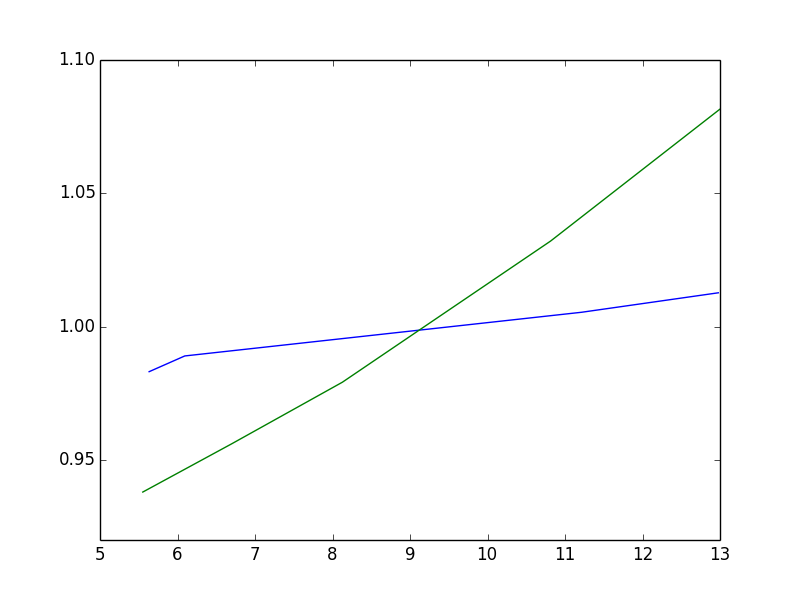
\includegraphics[width=0.6\linewidth]{delka_perioda.png}
            \caption{Změřená závislost periody na poloze těžiště pro obě osy kyvadla}
        \end{figure}

        \paragraph{} Odměřením průniku vygenerovaných křivek získám hledanou polohu těžiště.

        \begin{equation}
            y = 9.2306 cm
        \end{equation}

    \subsection{Měření doby kyvů a redukované délky}

        \paragraph{} Pro změřenou polohu jsem zjistil následující dobu kyvů.

        \begin{equation}
            \frac{T}{2} = (0.99776 \pm 7.2242 \cdot 10^{-6}) s
        \end{equation}

        Redukovaná délka (vzdálenost os) je po změření 

        \begin{equation}
            l = (98.9 \pm 0.05) cm
        \end{equation}

    \subsection{Výsledné tíhové zrychlení}

        \paragraph{} Ze vztahu (1) lze nyní stanovit hodnotu tíhového zrychlení
        a výchází následovně.

        \begin{equation}
            g = (9.805 \pm 0.003) m \cdot s^{-1}
        \end{equation}

        \paragraph{} 

\section{Výsledky}

    \paragraph{} S ohledem na uváděnou hodnota tíhového zrychlení pro brno
    $g_{Brno} = 9.81275 m \cdot s^{-1}$ je hodnota zjištěná v tomto měření
    poměrně přesná, od uváděné se liší pouze o $0.007 m \cdot s^{-1}$.

\end{document}
